\section{\scshape Introduction}
\subsection{Probabilistic Automata}

\begin{frame}
	\begin{center}
		\Large{Learning Probabilistic Automata}
		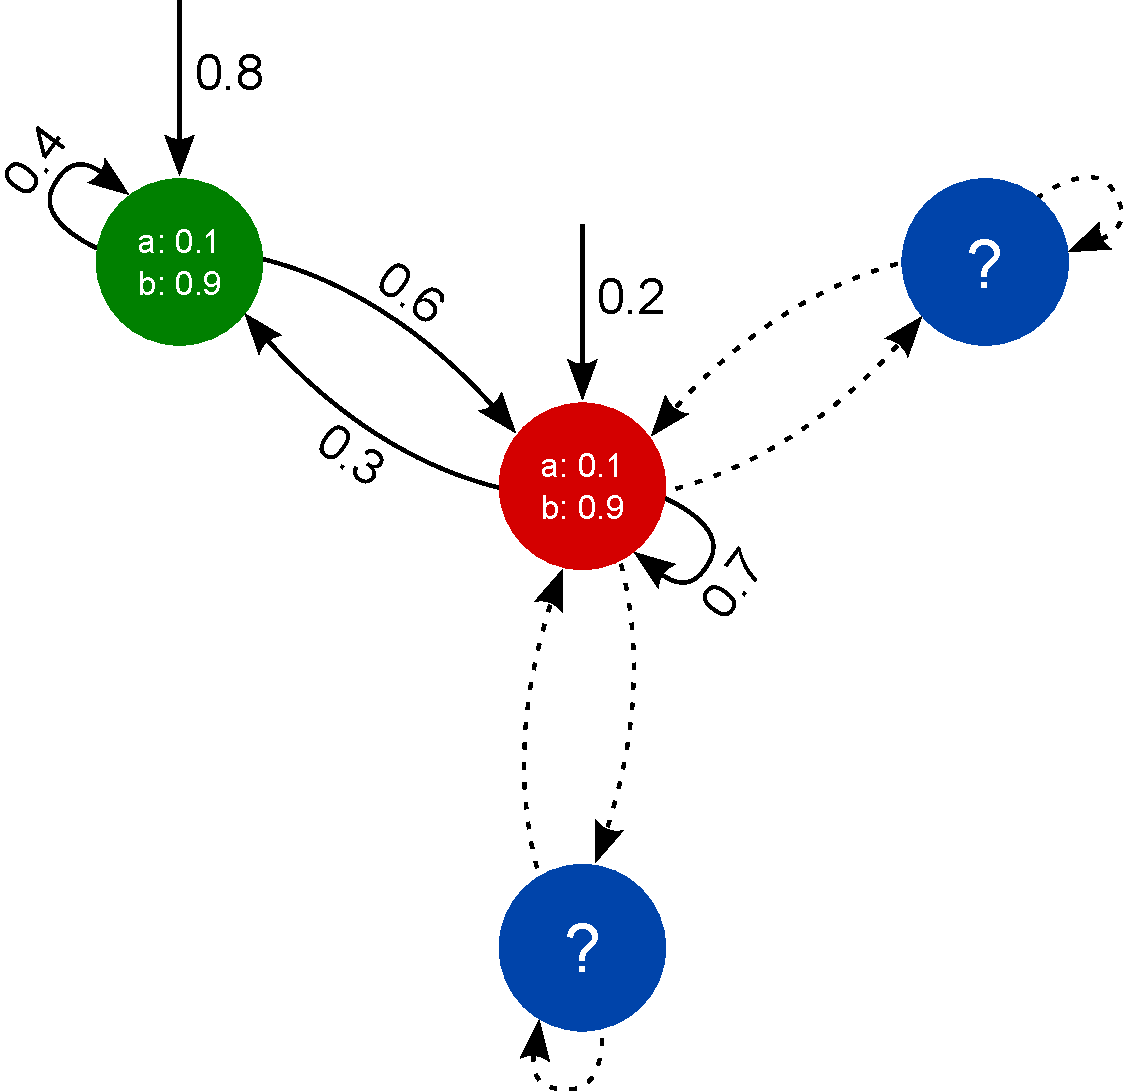
\includegraphics[width=0.48\textwidth]{images/frontpagemodel.pdf}\\
		\small{\textbf{Mathias M. Andersen\\
		Kent M. Caspersen\\
		Anders R. Nielsen\\
		Juraj Kol\v{c}\'{a}k\\
		Guillaume Grippari\\
		Theis Christensen\\}}
	\end{center}
\end{frame}

\begin{frame}
	\begin{center}
		\frametitle{Models}
		
		$$n~grams \approx Markov~chains \leq DPFA...\leq$$
		
		$$\leq HMM \approx PFA\leq$$
		
		$$\leq Multiplicity~automata$$
	\end{center}
\end{frame}

\subsection{PAutomaC}

\begin{frame}
	\frametitle{\emph{PAutomaC}}
	\begin{itemize}
		\item 2012 online PFA learning competition.
		\item All results and training data published after competition finished.
		\item Large amount of data available artificially generated by several types of models (Markov chains, DPFA, PFA, HMM).
		\item The generator models vary in number of states/symbols and density of the transitions and emissions providing for a large scale of different data.
	\end{itemize}
\end{frame}

\subsection{Problem Definition}

\begin{frame}
	\begin{center}
		\frametitle{Problem Definition}
		
		``Based on the \emph{PAutomaC} competition data, how can we learn not only the probabilistic parameters but the the structure of an HMM as well.''
	\end{center}
\end{frame}

\section{Analysis}
\subsection{Hidden Markov Models}

\begin{frame}
\center \huge \scshape Hidden Markov Models
\end{frame}

\begin{frame}
	\frametitle{Definition}
	
	Alphabet of observable symbols $\Sigma = \{\sigma_1, ..., \sigma_m\}$.\\
	Set of hidden states $S = \{s_1, ..., s_n\}$.
	
	Sequence of observable symbols $\mathbf{O}=(o_1,...,o_T)=\Sigma^T$.\\
	Sequence of hidden states $\mathbf{Q}=(q_1,....,q_T)=S^T$.
	
	$$\lambda=(\mathbf{A},\mathbf{B},\boldsymbol{\pi})$$
	
	Transition matrix $\mathbf{A}$: $\forall s,r\in S: a_{sr}=P(q_{t+1}=r|q_t=s)$\\
	Emission matrix $\mathbf{B}$: $\forall s\in S, \forall \sigma\in\Sigma: b_{s}(\sigma)=P(o_t=\sigma|q_t=s)$\\
	Initial probability distribution $\boldsymbol{\pi}$: $\forall s\in S:\boldsymbol{\pi}_s=P(q_1=s)$
\end{frame}

\begin{frame}
	\frametitle{Evaluation}
	
	Validation signal $\mathbf{O}=(o_1,...,o_T)$ and model $\lambda$.
	
	\begin{align*}
		P(\mathbf{O}|\lambda)&=\sum_{\mathbf{Q}\in\mathcal{Q}^T_\lambda}{P(\mathbf{O}|\mathbf{Q},\lambda)P(\mathbf{Q}|\lambda)}\\
		&=\sum_{\mathbf{Q}\in\mathcal{Q}^T_\lambda}{\pi_{q_1}b_{q_1}(o_1)a_{q_1q_2}b_{q_2}(o_2)...a_{q_{T-1}q_T}b_{q_T}(o_T)}
	\end{align*}
\end{frame}

\begin{frame}
	\frametitle{Forward-Backward Procedure}
	
	Forward variable:
	\begin{align*}
		\forall s\in S&: \alpha_1(s)=\pi_sb_{s}(o_1)\\
		\forall s\in S, t\in\{2, ..., T\}&: \alpha_t(s) = \sum_{r \in S}{(\alpha_{t-1}(r)a_{rs})}b_{s}(o_t)
	\end{align*}
	
	Backward variable:
	\begin{align*}
		\forall s\in S&:\beta_T(s)=1\\
		\forall s\in S, t\in\{1, ..., T-1\}&:\beta_t(s)=\sum_{r\in S}{(a_{sr}b_{r}(o_{t+1})\beta_{t+1}(r))}
	\end{align*}
	
	$$\sum_{s\in S}{\alpha_T(s)} = P(\mathbf{O}|\lambda)=\sum_{s\in S}{\beta_1(s)}$$
	
\end{frame}

\begin{frame}
	\frametitle{Baum-Welch Algorithm}
	
	$$\forall t\in\{1,...,T-1\},\forall s,r\in S: \xi_t(s,r) = P(q_t =s, q_{t+1}=r|\mathbf{O},\lambda)=$$
	$$=\frac{\alpha_t(i)a_{sr}b_{r}(o_{t+1})\beta_{t+1}(r)}{\sum_{u\in S}\sum_{v\in S}(\alpha_t(u)a_{uv}b_{v}(o_{t+1})\beta_{t+1}(v))}$$
		
	$$\forall t\in\{1,...,T\},\forall s\in S: \gamma_t(s) =P(q_t=s|\mathbf{O},\lambda)=\sum_{r\in S}\xi_t(s,r)$$
\end{frame}

\begin{frame}
	\frametitle{Baum-Welch Algorithm}
	
	\begin{align*}
		\forall s\in S: \overline{\pi_s} &= \gamma_1(s)\\
		\forall s,r\in S: \overline{a_{sr}} &= \frac{\sum_{t=1}^{T-1}\xi_t(s,r)}{\sum_{t=1}^{T-1}\sum_{u\in S}\xi_t(s,u)}\\
		\forall s\in S,\forall \sigma\in\Sigma:\overline{b_{s}(\sigma)}&=\frac{\sum_{t\in\mathcal{T}_\mathbf{O}(\sigma)}\gamma_t(s)}{\sum_{t=1}^T\gamma_t(s)}
	\end{align*}
	$$\mathcal{T}_\mathbf{O}(\sigma) = \{t\in\{1,...,T\}|o_t=\sigma\}$$
	
	$$P(\mathbf{O}|\overline{\lambda}=(\mathbf{\overline{A}}, \mathbf{\overline{B}}, \boldsymbol{\overline{\pi}})) >= P(\mathbf{O}|\lambda=(\mathbf{A}, \mathbf{B}, \boldsymbol{\pi}))$$
\end{frame}

\begin{frame}
	\frametitle{HMM vs PFA}
	
	\begin{itemize}
		\item HMMs and PFAs are mutually convertible between each other.
		\item PFAs often utilise stopping probabilities (also used for \emph{PAutomaC} models).
		\item Distribution defined by PFA with stopping probabilities: $P(\Sigma^*)$ against the HMM: $\forall n\in \mathbb{N}:P(\Sigma^n)$.
		\item A possible solution: introduce a new ``stopping'' symbol $x\notin\Sigma$ and create an HMM over the alphabet $\overline{\Sigma}=\Sigma\cup\{x\}$. End the signal once the new symbol $x$ is reached.
	\end{itemize}
\end{frame}

\begin{frame}
	\frametitle{HMM Density}
	
	\begin{itemize}
		\item Empirical results show that real world entities display ``sparse'' behaviour.
		\item Current state-of-the-art methods (Baum-Welch for HMMs) require the user to fully specify the amount of states and structure of the transition graph.
		\item Sparse transition matrix can also provide for a computational speedup.
	\end{itemize}
\end{frame}